\subsection{DCモータのモデリング}
DCモータの代表的な等価回路を\refig{dcm_circit}に示す.\cite{dcmmodeling}ただし,モータへの入力電圧を$v\unit{V}$,電機子電流を$i_{a}\unit{A}$,電機子抵抗を$R_{a}\unit{\Omega}$,自己インダクタンスを$L_{a}\unit{H}$,誘起電圧定数を$K_{E}\unit{Vs/rad}$,電機子の回転角速度を$\omega_{m}\unit{rad/s}$,電機子に発生するトルクを$T\unit{Nm}$,負荷トルクを$T_L\unit{Nm}$,回転子と負荷の合成慣性モーメントを$J\unit{kg\cdot m^2}$とする.以下ではこの等価回路に沿ってDCモータの定式化を行う.

\refig{dcm_circit}より,DCモータの支配方程式は次のように書ける.
\begin{align}
v &= K_{E}\omega_{m} + R_{a}i_{a} + L_{a}\frac{di_{a}}{dt} \label{eq::dcm_v} \\
T &= J\frac{d\omega_{m}}{dt} + T_{L} \label{eq::dcm_t}
\end{align}

\refeq{dcm_v},\refeq{dcm_t}より\refig{dcm_block}のブロック線図を得る.
ここで,図中の$J$はモータ回転子の慣性モーメント$J_{M}$と負荷の慣性モーメント$J_{L}$の和を表し,
$K_{T}\unit{Nm/A}$はDCモータのトルク定数である.
\refig{dcm_block}より負荷を含まないDCモータ単体の伝達関数$G_{M}(s)$を求めると以下のようになる.
\begin{align}
G_{M}(s) &= \frac{\Omega_{m}(s)}{V(s)} = 
\frac{\cfrac{K_{T}}{(R_{a} + L_{a}s)J_{M}s}}{1 + \cfrac{K_{T}K_{E}}{(R_{a} + L_{a}s)J_{M}s}} \nonumber \\
 &= \frac{\cfrac{1}{K_{E}}}{1 + \cfrac{R_{a}J_{M}}{K_{T}K_{E}}s + \cfrac{L_{a}J_{M}}{K_{T}K_{E}}s^2} \label{eq::dcm_tf}
\end{align}

ただし,$\Omega_{m}(s) = \mathcal{L}\{\omega_{m}(t)\},V(s) = \mathcal{L}\{v(t)\}$である.

\refeq{dcm_tf}より,電流の増加を遅らせるインダクタンスと回転角速度の上昇を遅らせる慣性モーメントという2つのエネルギ蓄積素子が二次のダイナミクスをつくっている事がわかる.

\begin{figure}[htb]
  \centering
    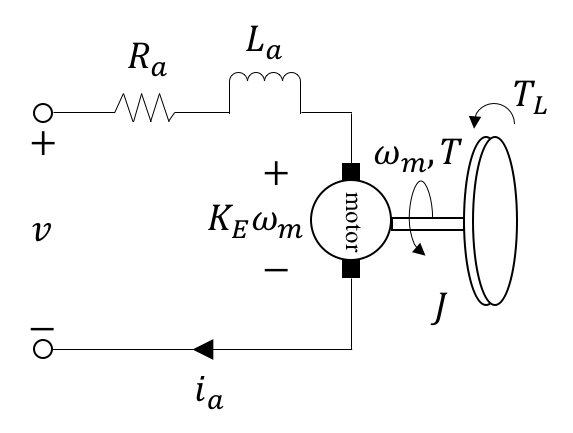
\includegraphics[width=0.5\hsize]{picture/eps/dcm_circit.eps}
    \caption{DCモータの等価回路}
    \label{fig::dcm_circit}
\end{figure}

\begin{figure}[htb]
  \centering
    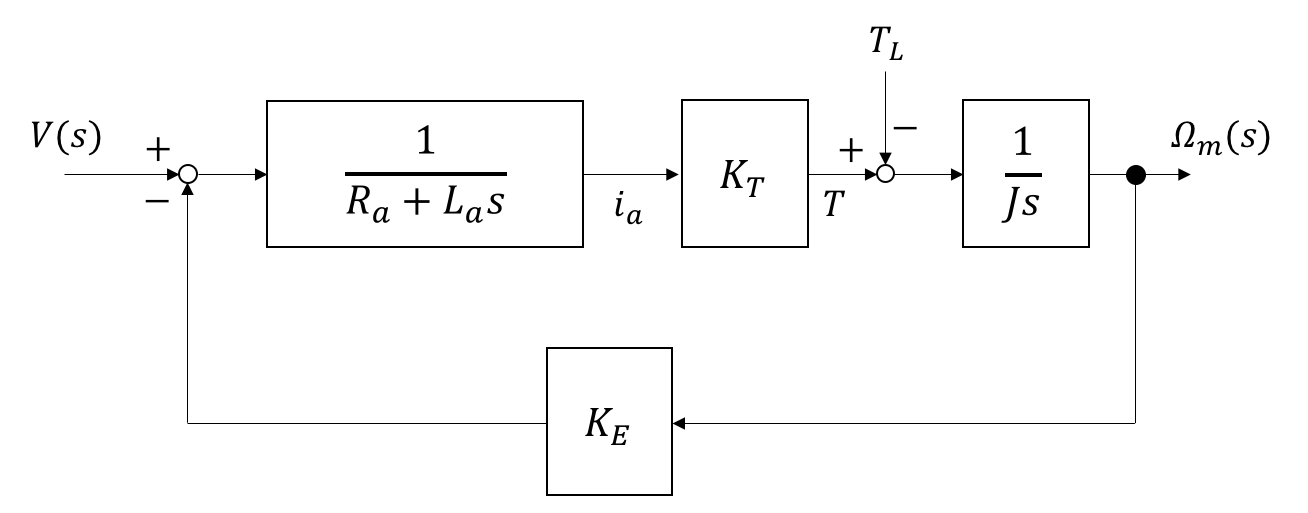
\includegraphics[width=1.0\hsize]{picture/eps/dcm_block_diagram.eps}
    \caption{DCモータのブロック線図}
    \label{fig::dcm_block}
\end{figure}
